% Symmetry defect operator deformation past a charged local operator.
% Left panel: U_g(Sigma) to one side of O(x).
% Right panel: U_g(Sigma') has swept past O(x), yielding g.O(x).
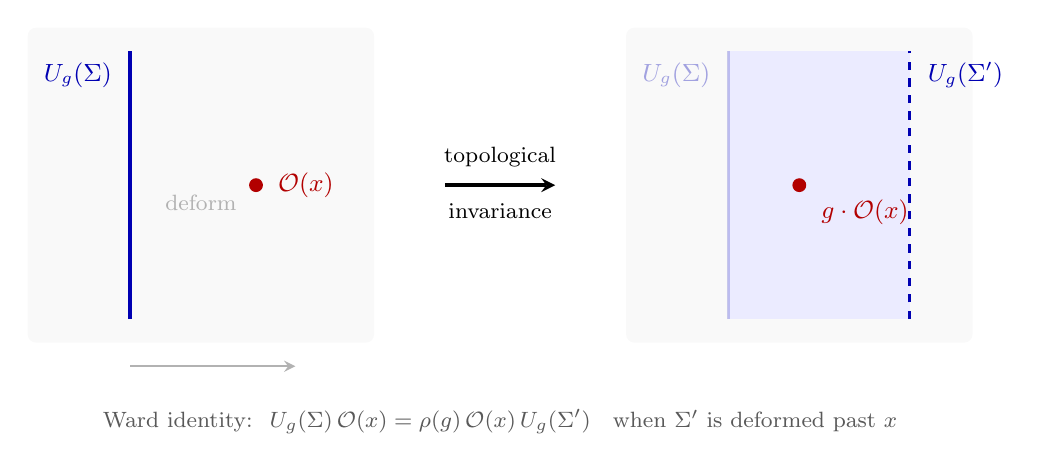
\begin{tikzpicture}[thick,
    defect/.style={very thick, blue!70!black},
    defect prime/.style={very thick, blue!70!black, dashed},
    operator/.style={fill=red!70!black, inner sep=0pt, minimum size=5pt, circle},
    arrow label/.style={font=\large, midway, above}]

  % ===== Left panel =====
  \begin{scope}[shift={(-3.8, 0)}]
    % Spacetime region (light gray background)
    \fill[gray!5, rounded corners=3pt] (-2.2, -2.0) rectangle (2.2, 2.0);

    % Codimension-1 defect surface Sigma (vertical line in 2d slice)
    \draw[defect] (-0.9, -1.7) -- (-0.9, 1.7);
    \node[blue!70!black, font=\small, anchor=east] at (-1.0, 1.4) {$U_g(\Sigma)$};

    % Charged local operator
    \node[operator] (Ox1) at (0.7, 0) {};
    \node[red!70!black, font=\small, anchor=west] at (0.85, 0) {$\mathcal{O}(x)$};

    % Arrow indicating deformation direction
    \draw[->, >=stealth, gray!60, thick]
      (-0.9, -2.3) -- (1.2, -2.3);
    \node[gray!60, font=\footnotesize, below, midway] at (0.15, -2.3) {deform};
  \end{scope}

  % ===== Central arrow =====
  \draw[->, >=stealth, line width=1.2pt] (-0.7, 0) -- (0.7, 0);
  \node[font=\footnotesize, above] at (0, 0.1) {topological};
  \node[font=\footnotesize, below] at (0, -0.1) {invariance};

  % ===== Right panel =====
  \begin{scope}[shift={(3.8, 0)}]
    % Spacetime region
    \fill[gray!5, rounded corners=3pt] (-2.2, -2.0) rectangle (2.2, 2.0);

    % Shaded region swept by deformation (drawn first, behind everything)
    \fill[blue!8] (-0.9, -1.7) rectangle (1.4, 1.7);

    % Original position (ghost)
    \draw[defect, opacity=0.2] (-0.9, -1.7) -- (-0.9, 1.7);
    \node[blue!70!black, font=\small, anchor=east, opacity=0.35]
      at (-1.0, 1.4) {$U_g(\Sigma)$};

    % Deformed defect surface Sigma' (new position, past the operator)
    \draw[defect prime] (1.4, -1.7) -- (1.4, 1.7);
    \node[blue!70!black, font=\small, anchor=west] at (1.5, 1.4) {$U_g(\Sigma')$};

    % Charged local operator — now acted on by g
    \node[operator] (Ox2) at (0.0, 0) {};
    \node[red!70!black, font=\small, anchor=west] at (0.15, -0.35)
      {$g \cdot \mathcal{O}(x)$};
  \end{scope}

  % ===== Ward identity annotation =====
  \node[font=\footnotesize, gray!70!black, align=center] at (0, -3.0)
    {Ward identity:\;
     $\displaystyle U_g(\Sigma)\,\mathcal{O}(x)
       = \rho(g)\,\mathcal{O}(x)\,U_g(\Sigma')$
     \; when $\Sigma'$ is deformed past $x$};

\end{tikzpicture}
